\documentclass[12pt]{article}
\usepackage[T1]{fontenc}
\usepackage[utf8]{inputenc}
\usepackage{url}
\usepackage{enumerate}
\usepackage[top=3cm, bottom=3cm]{geometry}
\usepackage{graphicx} 
\usepackage{enumitem}
\usepackage{natbib}
\usepackage{listings}
\usepackage{float}
\usepackage{amsmath}
\usepackage{color}
\bibpunct{[}{]}{,}{a}{}{;}
\setcitestyle{super}

% Variables
\newcommand{\assignmentname}{Assignment 1}
\newcommand{\coursename}{Advanced Algorithms and Data Structures}
\newcommand{\studentname}{Bjarki Madsen (lch929) - Michael Bang (??)}
\newcommand{\department}{Department of Computer Science}
\newcommand{\institution}{Copenhagen University}
\newcommand{\location}{Copenhagen, Denmark}

\begin{document}

\renewcommand\refname{References}

\title{\assignmentname \\ {\Large {\textsc \coursename}}}
\author{
        \studentname \\
        \department \\
        \institution \\
        \location
}
\date{\today}

\maketitle
\thispagestyle{empty}

\pagebreak

\section*{Exercise 1}

  Figure \ref{fig:e1_a_solution} shows a b-flow with maximum value of 9 for the first proposed graph from the assignment. The second proposed graph from the assignment has no b-flow. The reason is that $v_1$ wants to have at least $3 + c(v_2, v_1)$ after giving away $f(v_1, v_3)$. In order for that to happen the $f(v_2, v_1)$ has to equal to $c(v_2, v_1)$. After the $f(v_2, v_1)$, $v_2$ wants to end up with 1 in demand, meaning it needs a flow value of 4 to itself but that is impossible because the maximum flow to $v_2$ is equal to $c(v_3, v_2)$, or 2 and therefore is unable to fulfill $f(v_2, v_1) = c(v_2, v_1)$. 

  \begin{figure}[h]
    \centering
      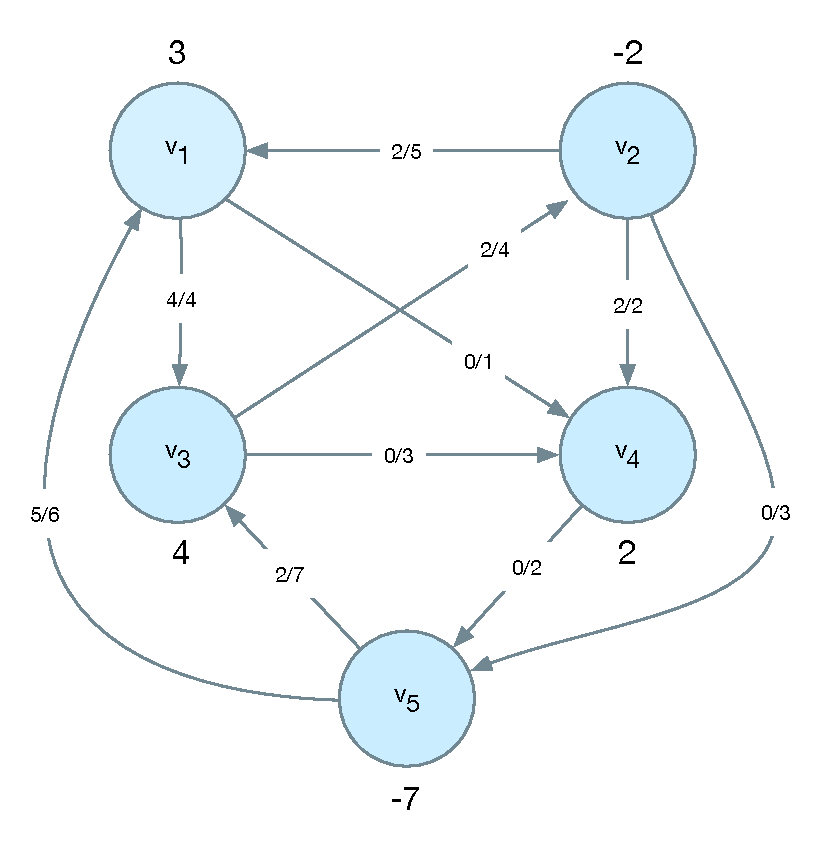
\includegraphics[width=0.6\textwidth]{figures/e1_a_solution}
    \caption{Graph showing b-flow with maximum flow = 9}
    \label{fig:e1_a_solution}
  \end{figure}

\end{document}
% End of document.







